\documentclass[10pt,a4paper]{article}

\usepackage[utf8]{inputenc}
\usepackage[T1]{fontenc}
\usepackage[french]{babel}

%format de la page%
\usepackage{geometry}
\geometry{hmargin=2.5cm,vmargin=2.5cm}

%style des headers/footers%
\usepackage{lastpage}
\usepackage{fancyhdr}
\pagestyle{fancy}

\renewcommand{\headrulewidth}{1pt}
\fancyhead[C]{} 
\fancyhead[L]{\leftmark}
\fancyhead[R]{}

\renewcommand{\footrulewidth}{1pt}
\fancyfoot[C]{\textbf{\thepage/\pageref{LastPage}}} 
\fancyfoot[L]{Réseau}
\fancyfoot[R]{Alexandre Kornmann}

%packages maths%
\usepackage{amsmath}
\usepackage{amsfonts}
\usepackage{amssymb}

\newcommand{\N}{{\mathbb{N}}}
\newcommand{\Z}{{\mathbb{Z}}}
\newcommand{\R}{{\mathbb{R}}}


%affichage de code source%
\usepackage{listings}

\lstset{
language=fortran,
frame=single,
keywordstyle=\color{blue}\bfseries,
commentstyle=\color{green}\itshape,
stringstyle=\color{red},
showstringspaces=false,
breaklines=true,
breakatwhitespace=true}

%divers%
\usepackage{caption}
\usepackage{url}
\usepackage{subfig}
\usepackage[colorlinks=true,urlcolor=blue]{hyperref}
\usepackage{float}
\usepackage{graphicx}


\title{Projet réseau}
\author{Alexandre Kornmann}

\begin{document}

\maketitle

\newpage

\tableofcontents

\newpage

\section{Documentation utilisateur}
\subsection{Démarage d'un client}

Le client démarre par la commande
\begin{center}
\fbox{./PRAK client} 
\end{center}

\subsection{Démarage d'un serveur}

Le client démarre par la commande
\begin{center}
\fbox{./PRAK server xxxx}
\end{center}avec xxxx, un port libre sur la machine courante. 

\textit{Il faut démarrer chaque serveur dans un \textbf{dossier différent}, afin que chacun est ses propres fichiers, et afin d'éviter tout comportement indésirable.}
\subsection{Liste des commandes clients}

\subsubsection{catalogue}
\begin{center}
\fbox{catalogue} 
\end{center}
\textbf{catalogue} (ou son alias \textbf{lib}) affiche la bibliotèque sur la sortie standard.

\subsubsection{lire}
\begin{center}
\fbox{lire FICHIER} 
\end{center}
\textbf{lire} (ou son alias \textbf{dl}) affiche le fichier FICHIER sur la sortie standard.

\subsubsection{stocker}
\begin{center}
\fbox{stocker FICHIER TITRE} 
\end{center}
\textbf{stocker} (ou son alias \textbf{ul}) ajoute le fichier FICHIER sur deux serveurs, et l'ajoute catalogue sous le titre TITRE. FICHIER doit se trouver dans le dossier où a été lancé l'application client.

\subsubsection{detruire}
\begin{center}
\fbox{detruire NOMFICHIER} 
\end{center}
\textbf{detruire} (ou son alias \textbf{rm}) détruit le fichier FICHIER de tout les serveurs, et le retire du catalogue.

\subsubsection{exit}
\begin{center}
\fbox{exit}
\end{center}
\textbf{exit} quitte le client.

\subsection{Fichier de configuration}

Le format d'une ligne du fichier du configuration qui contient la liste de tout les serveurs à contacter est le suivant :
\begin{center}
\fbox{NOMHOTE|IPV4|IPV6 PORT}
\end{center}
Chaque ligne contient un enregistrement du type IP espace PORT, ou HOTE espace PORT.\\
\textit{Attention : ne pas laisser de ligne vide à la fin du fichier, ou d'espace inutile en fin de ligne.}\\

Exemple :\\
127.0.0.1 4242\\
turing.u-strasbg.fr 5254\\
turing.u-strasbg.fr 4024\\
\newpage

\section{Protocoles}

\subsection{Philosophie des protocoles}
Tout les protocoles suivants sont basés sur une philosophie commune : le client demande, le serveur répond.
Le serveur ne peut pas prendre d'initiative dans une transaction, il se contente de réagir aux demandes du client.
\subsection{Format du datagramme}

Le datagramme qui permet la communication est de la forme :
\begin{enumerate}
 \item int : \textbf{code}
 \item int : \textbf{seq}
 \item 512 char : \textbf{data}
\end{enumerate}

Par la suite, on notera un datagramme de la façon suivante :

\begin{center}
 \fbox{\textbf{dg(code,seq,data)}}
\end{center}

Des paramètres peuvent être omis.

\vspace{0.3cm}
\textbf{code} permet donc d'identifier à quoi correspond la suite du datagramme.
\textbf{code} peut prendre sa valeur entre 0 et 6, ce qui correspond au type de paquet suivants :
\begin{itemize}
 \item 0 = CONNECTRA
 \item 1 = DISCONNECTRA
 \item 2 = DOWNLOAD
 \item 3 = UPLOAD
 \item 4 = ADD
 \item 5 = REMOVE
 \item 6 = GET
\end{itemize}

\subsection{CONNECTRA : Requête de connexion d'un client à un serveur}
Ce protocole très simple permet de signifier à un serveur qu'on souhaite entamer une transaction avec le serveur.
Le client envoie \textbf{dg(0,0,)}. Le serveur répond \textbf{dg(0,1,)}.

\subsection{DISCONNECTRA : Requête de déconnexion d'un client à un serveur}
Ce protocole très simple permet de signifier à un serveur qu'on souhaite mettre un terme à une transaction avec le serveur.
Le client envoie \textbf{dg(1,1,)}. Le serveur répond \textbf{dg(1,0,)}.

\subsection{DOWNLOAD : Récupération d'un fichier présent sur le serveur}
Pour initier la transaction, le client envoie le paquet \textbf{dg(2,0,nom du fichier)}.
Les réponses possibles sont :
\begin{itemize}
 \item \textbf{dg(2,2,)} : Le fichier est dans la librairie et est disponible sur le serveur.
 \item \textbf{dg(2,1,)} : Le fichier est dans la librairie mais n'est pas disponible sur le serveur.
 \item \textbf{dg(2,0,)} : Le fichier n'est pas dans la bibliotèque
\end{itemize}

En fonction de cette réponse, le client peut décider de demander le fichier, avec \textbf{dg(2,0,nom du fichier)}
Si le serveur trouve le fichier, il va répondre avec la taille du fichier en numéro de séquence, sinon le serveur répond 0 en numéro de séquence.
Par la suite le client envoie au serveur des paquets de la forme \textbf{dg(2,x,)}, avec \textbf{x} l'indice du dernier caractère du fichier que l'on souhaite recevoir.
La fin du transfert est signifié à la réception d'un paquet contenant moins de 512 caractères.

\subsubsection{Motivation des choix}
Ce choix de protocole est proche dans l'esprit du protocole TFTP (RFC 1350), et relativement simple à implémenter. Il génère cependant beaucoup d'acquittements superflus.
\subsubsection{Autre solution}
On pourrait limiter le nombre d'acquittements en se contentant d'envoyer la taille du fichier, l'acquitter, puis le fichier en entier, et acquitter la totalité du fichier. Si des paquets sont perdus, le client peut, connaissant la taille du fichier, déterminer lesquelles sont manquant et en faire la demande explicite.


\subsection{UPLOAD : Envoi d'un fichier sur un serveur}
Pour initier la transaction, le client envoie le paquet \textbf{dg(3,x,)} et recoit en acquittement le paquet \textbf{dg(3,x,)}.
Ensuite, le client envoie trois paquets contenant les métadonnées : \textbf{dg(3,0,nom du fichier)}, \textbf{dg(3,1,titre du fichier)}, et \textbf{dg(3,taille du fichier,)}. Le serveur acquitte les trois en renvoyant \textbf{dg(3,taille du fichier,)}.
Pour le transfert des données, le client envoie un paquet contenant 512 caractères, \textbf{dg(3,seq,chaine de 512 caractères)} que le serveur acquitte par \textbf{dg(3,seq,)}.
Un paquet de longueur inférieur à 512 signifie la fin de la transaction. \textbf{seq} indique la position du dernier caractères de la chaîne dans le fichier.

\subsubsection{Motivation des choix}
On pourrait d'abord penser que le transfert de fichier se fait de manière symétrique de client à serveur et de serveur à client. Mais celà impliquerai que le serveur devienne ``actif'', et qu'il gère lui aussi des timeouts.

\begin{figure}[H]
 \centering
 \includegraphics[width=7cm]{Diagramme6}
 \caption{Représentation schématique du protocole UPLOAD}
\end{figure}

\subsection{ADD : ajout d'un fichier à la bibliotèque}
Afin d'ajouter un fichier à la bibliotèque, le client envoie deux paquets contenant respectivement le nom du fichier et son titre (\textbf{dg(4,0,nom du fichier)} et \textbf{dg(4,1,titre du fichier)}).

Le serveur acquitte chaque paquet en répondant avec le même numéro de séquence que le paquet recu (c'est à dire \textbf{dg(4,0,)} ou \textbf{dg(4,1,)})

\subsection{REMOVE : retrait d'un fichier de la bibliotèque}
Afin de retirer un fichier de la bibliotèque, le client envoie un paquet \textbf{dg(5,0,nom du fichier)}.
Le serveur acquitte chaque paquet en répondant \textbf{dg(5,0,)}.

\subsection{GET : récupération de l'intégralité de la bibliotèque}
Afin d'initier la transaction, le client envoie un paquet \textbf{dg(6,0,)}.
Le serveur répond alors \textbf{dg(6,lignes,)} avec \textbf{lignes} le nombre d'entrée dans la bibliotèque.
Le client peut alors demander la ième ligne de la bibliotèque (avec \textbf{dg(6,i,)}). Le serveur répond alors en envoyant deux paquets contenant respectivement un nom de fichier et le titre associé (\textbf{dg(6,i,nom du fichier)} et \textbf{dg(6,i+lignes,titre})).

\newpage

\section{Architecture}
\subsection{Idée générale}
Le projet se divise en (paires de) fichiers, chacune contenant une classe ou une structure de donnée. Chaque classe fournit des services. L'implémentation essaie de respecter au mieux le paradigme oritenté objet.

En résumé :
\begin{itemize}
 \item \textbf{addr\_map} : structure de donnée permettant de lier une adresse à un état (voir \ref{sec:etat})
 \item \textbf{AddrStorage} : encapsulation de la couche communication (voir \ref{sec:communication}), élément de addr\_map
 \item \textbf{Client} : partie client, offre les services lire/stocker/détruire/catalogue.
 \item \textbf{Converter} : classe outil permettant des conversions de type et le découpage de chaîne de caractères
 \item \textbf{Counter} : compteur d'itération permettant le bloquage de la transaction
 \item \textbf{Datagram} : définition du format du datagramme servant aux transactions
 \item \textbf{Exception} : gestion d'exceptions
 \item \textbf{File} : offre des services de lecture et d'écriture dans un fichier
 \item \textbf{library} : structure de donnée permettant le stockage en mémoire du catalogue
 \item \textbf{main} : point d'entrée de l'application
 \item \textbf{Record} : élément due library
 \item \textbf{Server} : partie serveur du projet
 \item \textbf{Shell} : invite de commande permettant d'utiliser les services du client
 \item \textbf{socket} : définition de quelques macros, contient les librairies nécessaire dans tout le projet
 \item \textbf{State} : état d'une transaction, élément de addr\_map
\end{itemize}

\subsection{Serveur est un client}
Dans certains cas, comme lorsque un serveur devient dépositaire d'un nouveau fichier, le serveur à un comportement très proche voir identique à un client. C'est pour ca que le serveur est un client à part entière, ce qui se traduit par la notion d'héritage en C++.

\begin{figure}[H]
 \centering
 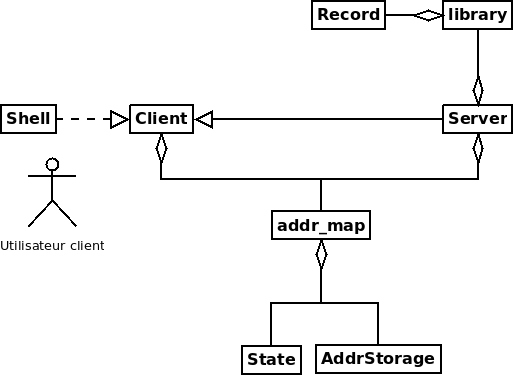
\includegraphics[width=12cm]{Diagramme1}
 \caption{Schéma de l'organisation des composants}
\end{figure}

\newpage
\subsection{Serveur à état} \label{sec:etat}
Un serveur sans état (stateless) est un serveur qui traite chaque requête indépendamment des précédentes. L'inconvénient est que chaque transaction doit contenir plus d'informations.\\
Par opposition, un serveur à état (statefull) conserve une trace des transactions en cours. L'implémentation est plus complexe, mais les transactions sont plus légères. Le choix de protocole qui a été fait oblige l'implémentation d'un serveur à état.
Il faut cependant être très attentif aux débuts et fin de transactions, car des déconnexion ``sauvages'' du client peuvent arrivées, et le serveur doit toujours rester dans un état cohérent.\\

La connaissance d'un paquet et de son émetteur permettront de déterminer une réponse unique à renvoyer. Ceci est traduit dans la structure addr\_map, qui relie un émetteur à son état.

\begin{figure}[H]
 \centering
 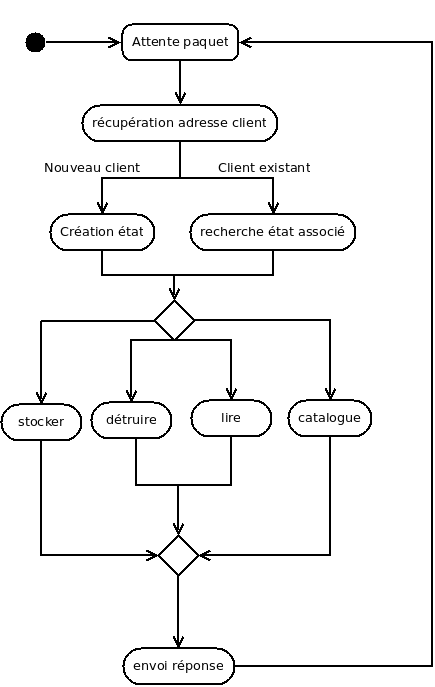
\includegraphics[width=8cm]{Diagramme3}
 \caption{Diagramme de fonctionnement du serveur}
\end{figure}

\subsection{Division en 3 couches}
L'application peut-être divisée en trois couches. En partant de la couche communication, qui encapsule toute la gestion des sockets, à la couche application, de plus haut niveau.
Chaque couche fait appel aux services offerts par la couche inférieur.
\begin{figure}[H]
 \centering
 \includegraphics[width=8cm]{Diagramme4}
 \caption{Séparation des couches dans la classe client}
\end{figure}
\subsubsection{Couche communication} \label{sec:communication}
Cette couche est relative à l'ensemble des tâches liées à la gestion des sockets et des adresses. Elle contient notamment la classe \textbf{AddrStorage} qui permet d'unifier le fonctionnement IPv4 et IPv6.
Cette couche contient également les méthodes du type \textbf{receive} et \textbf{send} des classes \textbf{Client} et \textbf{Server}. lEs constructeurs de ces deux dernières classes peuvent aussi être considéré dans cette couche, puisqu'ils déclarent les sockets. La méthode \textbf{run} du serveur quand a elle permet d'écouter sur les sockets, et fait donc partie de cette couche.
\subsubsection{Couche protocole}
Le contenu de cette couche est très simple à délimiter : elle contient tout les protocoles d'échanges (connexion, fichiers et bibliotèque).
\subsubsection{Couche application}
Les services offerts par cette couche sont ceux que l'utilisateur voit le plus directement : \textbf{get\_file} (lire), \textbf{send\_file} (stocker), \textbf{remove\_file} (détruire), \textbf{get\_library} (catalogue).


\end{document}

